% Options for packages loaded elsewhere
\PassOptionsToPackage{unicode}{hyperref}
\PassOptionsToPackage{hyphens}{url}
%
\documentclass[
]{article}
\usepackage{amsmath,amssymb}
\usepackage{iftex}
\ifPDFTeX
  \usepackage[T1]{fontenc}
  \usepackage[utf8]{inputenc}
  \usepackage{textcomp} % provide euro and other symbols
\else % if luatex or xetex
  \usepackage{unicode-math} % this also loads fontspec
  \defaultfontfeatures{Scale=MatchLowercase}
  \defaultfontfeatures[\rmfamily]{Ligatures=TeX,Scale=1}
\fi
\usepackage{lmodern}
\ifPDFTeX\else
  % xetex/luatex font selection
\fi
% Use upquote if available, for straight quotes in verbatim environments
\IfFileExists{upquote.sty}{\usepackage{upquote}}{}
\IfFileExists{microtype.sty}{% use microtype if available
  \usepackage[]{microtype}
  \UseMicrotypeSet[protrusion]{basicmath} % disable protrusion for tt fonts
}{}
\makeatletter
\@ifundefined{KOMAClassName}{% if non-KOMA class
  \IfFileExists{parskip.sty}{%
    \usepackage{parskip}
  }{% else
    \setlength{\parindent}{0pt}
    \setlength{\parskip}{6pt plus 2pt minus 1pt}}
}{% if KOMA class
  \KOMAoptions{parskip=half}}
\makeatother
\usepackage{xcolor}
\usepackage[margin=1in]{geometry}
\usepackage{graphicx}
\makeatletter
\def\maxwidth{\ifdim\Gin@nat@width>\linewidth\linewidth\else\Gin@nat@width\fi}
\def\maxheight{\ifdim\Gin@nat@height>\textheight\textheight\else\Gin@nat@height\fi}
\makeatother
% Scale images if necessary, so that they will not overflow the page
% margins by default, and it is still possible to overwrite the defaults
% using explicit options in \includegraphics[width, height, ...]{}
\setkeys{Gin}{width=\maxwidth,height=\maxheight,keepaspectratio}
% Set default figure placement to htbp
\makeatletter
\def\fps@figure{htbp}
\makeatother
\setlength{\emergencystretch}{3em} % prevent overfull lines
\providecommand{\tightlist}{%
  \setlength{\itemsep}{0pt}\setlength{\parskip}{0pt}}
\setcounter{secnumdepth}{-\maxdimen} % remove section numbering
\usepackage{booktabs}
\usepackage{wrapfig}
\usepackage{graphicx}
\usepackage{amssymb}
\usepackage{tikz}
\usepackage{amsmath}
\usepackage{color}
\usepackage{subcaption}
\usepackage[font=footnotesize]{caption}
\usepackage{titling}
\captionsetup[figure]{font=small}
                                          
\DeclareRobustCommand{\solidline}{\raisebox{2pt}{\tikz{\draw[thick](0,0) -- (0.5,0);}}}
\DeclareRobustCommand{\dashedline}{\raisebox{2pt}{\tikz{\draw[dashed, thick](0,0) -- (0.5,0);}}}                                          
\ifLuaTeX
  \usepackage{selnolig}  % disable illegal ligatures
\fi
\IfFileExists{bookmark.sty}{\usepackage{bookmark}}{\usepackage{hyperref}}
\IfFileExists{xurl.sty}{\usepackage{xurl}}{} % add URL line breaks if available
\urlstyle{same}
\hypersetup{
  hidelinks,
  pdfcreator={LaTeX via pandoc}}

\author{}
\date{\vspace{-2.5em}2024-05-15}

\begin{document}

\hypertarget{orion-star-ph-meter-cross-comparison-report}{%
\section{Orion Star pH Meter Cross Comparison
Report}\label{orion-star-ph-meter-cross-comparison-report}}

Sonya Havens\\
2024-05-31

\hypertarget{thermo-scientifictm-orion-startm-a211-benchtop-ph-meter}{%
\subsection{\texorpdfstring{Thermo Scientific\textsuperscript{TM} Orion
Star\textsuperscript{TM} A211 Benchtop pH
Meter}{Thermo ScientificTM Orion StarTM A211 Benchtop pH Meter}}\label{thermo-scientifictm-orion-startm-a211-benchtop-ph-meter}}

The Thermo Scientific\textsuperscript{TM} Orion Star\textsuperscript{TM}
A211 Benchtop pH Meter was purchased from Fisher Scientific 23 March
2023 and included the following parts''

\begin{itemize}
\tightlist
\item
  Star A211 pH meter
\item
  8172BNWP ROSS Sure-Flow glass-body pH electrode
\item
  927007MD stainless steel ATC probe
\item
  810199 pH buffer kit
\item
  electrode stand
\item
  100-240V universal power adapter
\item
  computer cable
\end{itemize}

The Thermo Scientific\textsuperscript{TM} Orion Star\textsuperscript{TM}
A211 pH Meter was received 7 April 2023, installed on 12 June 2023, and
used to measure pH in samples collected from 12 June 2023 to 6 September
2023 (\emph{n} = 301) that were also measured on the Fisher Accumet
Benchtop pH Meter. Samples from the Environment and Climate Change
Canada Proficiency Testing study (ECCC-PT) were also analyzed on the
Shimadzu HIC-ESP and compared with ECCC-PT results. Instrument
performance data (e.g.~detection limits and reference samples) is also
provided.

\hypertarget{precision}{%
\subsection{Precision}\label{precision}}

The analytical precision (\emph{Pr}), which is based on the residuals of
the standard buffers response along the calibration curve, is calculated
for each run using the measured response (mV) of standard buffers and
equations 1 through 3:

Equation 1. \(Pr = (y_d-b)/m\)

where \emph{b} is the y-intercept, \emph{m} is the slope, and
\emph{y\textsubscript{d}} is the signal detection limit, which is
calculated using equation 2.

Equation 2. \(y_d = 3s_y+b\)

where \emph{s\textsubscript{y}} is the residuals between the measured
response (mV) for each standard buffer and the calibration curve
predicted response (mV) for each standard concentration and is
calculated using equation 3.

Equation 3. \(s_y = √((∑d_i^2 )/(n-2))\)

where \emph{n} is the number of standards in the calibration curve, and
\emph{d\textsubscript{i}} is the difference between the measured
response (mV) for each standard buffer and the calibration curve
predicted response (mV) for each standard buffer.

The average analytical precision of pH measured on the Orion Star pH
meter and Fisher Accumet pH meter were similar (0.05 ± 0.03, \emph{n} =
37 and 0.03 ± 0.03, \emph{n} = 87, respectively).

\pagebreak

\hypertarget{reference-samples}{%
\subsection{Reference samples}\label{reference-samples}}

A reference sample is included in each analytical run. The average pH
result of reference samples measured on the Orion Star and Fisher
Accumet were similar (6.71 ± 0.11, \emph{n} = 37 and 6.65 ± 0.12,
\emph{n} = 87, respectively). The pH of the reference sample, measured
by both the Orion Star and Fisher Accumet pH meters, slowly declined
over time (, , for the Orion Star and Fisher Accumet pH meters,
respectively). This was likely due to CO\textsubscript{2} dissolution
into the reference sample bottle. The reference sample is lake 239
epilimnetic water that has been aged for at least one year prior to use
so that the chemical constituents can stabilize and come to equilibrium
with the atmosphere. These reference sample pH results reveal that the
sample must not be equilibrated with the atmosphere, which is likely due
to the large volume of the sample. Going forward the sample should be
stored with a large head space and inverted several times before use to
ensure that the sample is equilibrated with the atmosphere.

\begin{figure}[h]
  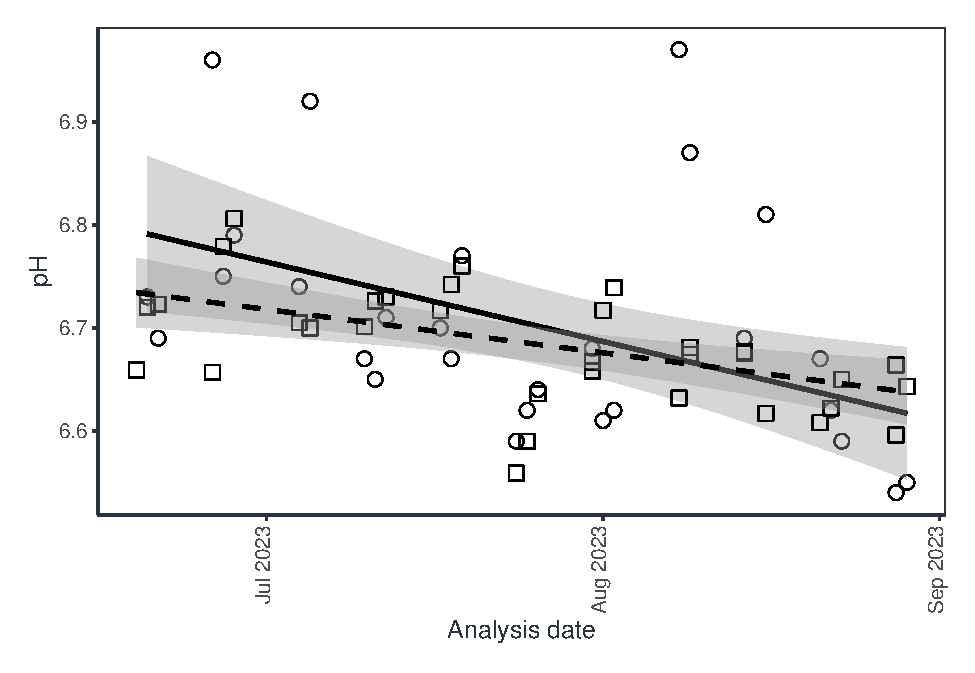
\includegraphics[width=0.5\textwidth]{ref_comparison_date.pdf}
  \caption{pH of reference sample measured with the Orion Star pH meter ($\bigcirc$, \protect\solidline, $\mbox{\textit{y} = 23}$$\mbox{-0.00083}$$\textit{x}$, $\mbox{\textit{n} = 39}$) and with the Fisher Accumet pH meter ($\square$, \protect\dashedline, $\mbox{\textit{y} = 33}$$\mbox{-0.0014}$$\textit{x}$, $\mbox{\textit{n} = 36}$) from June 2023 to September 2023}
\end{figure}

The pH results of reference samples were not well correlated among the
two pH meters (\emph{R\^{}2} = \texttt{ref\_fit\_rsquared}, \emph{p}
\textgreater{} 0.01) with the pH measured on the Orion Star pH meter
ranging from 6.54 to 6.97 and the pH measured on the Fisher Accumet pH
meter ranging from 6.379 to 6.85.

\ldots{}

\hypertarget{mv-stability}{%
\subsection{mV stability}\label{mv-stability}}

\begin{figure}[h]
  \begin{subfigure}{0.48\textwidth}
  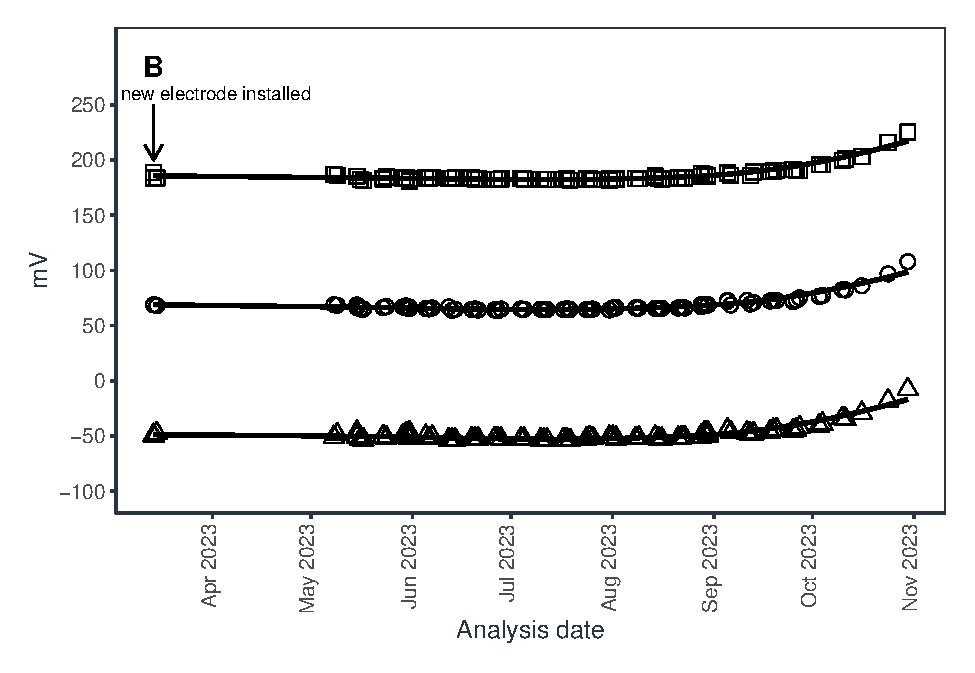
\includegraphics[]{fisher_mV.pdf}
  \end{subfigure}%
  \begin{subfigure}{0.48\textwidth}
  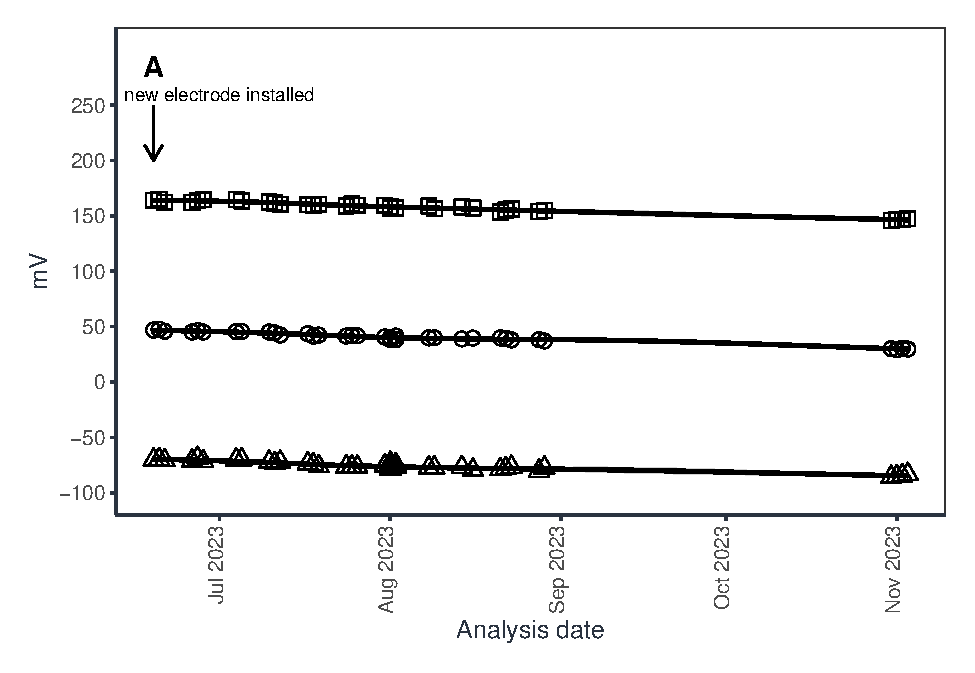
\includegraphics[]{orion_mV.pdf}
  \end{subfigure}
\caption{pH meter signal response (mV) of pH 4 ($\square$), pH 6 ($\bigcirc$), and pH 8 ($\bigtriangleup$) buffers from 19 June 2023 to 3 November 2023 for the Orion Star pH meter and from 14 March 2023 to 30 October 2023 for the Fisher Accumet pH meter}
\end{figure}

\hypertarget{slope}{%
\subsection{Slope}\label{slope}}

\begin{figure}[h]
  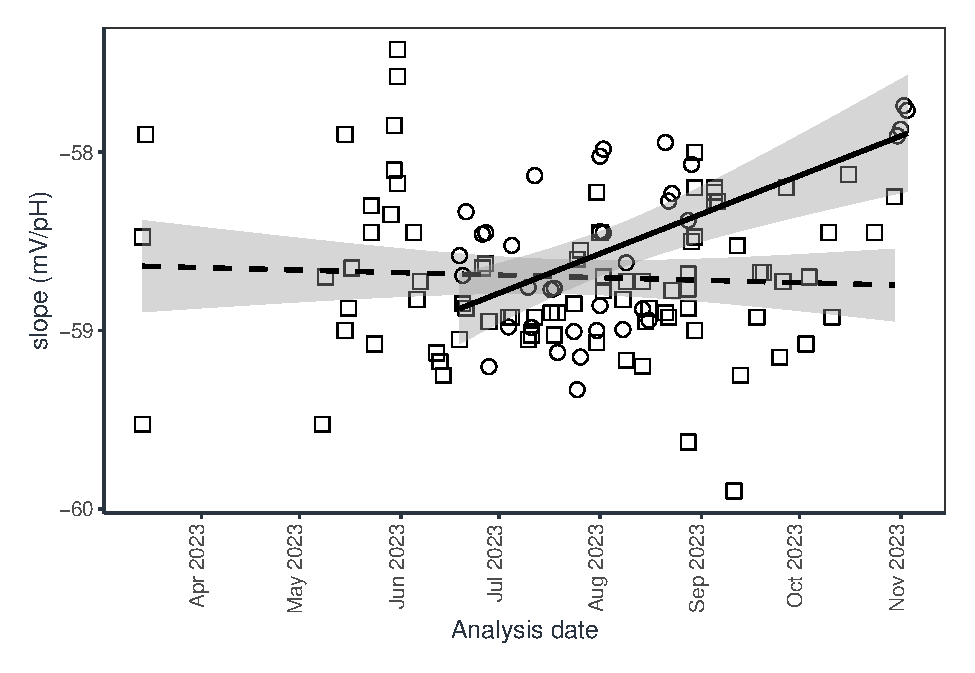
\includegraphics[width=0.5\textwidth]{mV_slope.pdf}
  \caption{Slope of pH meter calibrations of analytical runs on the Orion Star pH meter ($\bigcirc$, \protect\solidline, $\mbox{y = 23}$$\mbox{-0.0008}$$\textit{x}$, $\mbox{\textit{n} = 45}$) from 19 June 2023 to 3 November 2023 and with the Fisher Accumet pH meter ($\square$, \protect\dashedline, $\mbox{y = 33}$$\mbox{-0.0014}$$\textit{x}$, $\mbox{\textit{n} = 40}$) from 14 March 2023 to 30 October 2023}
\end{figure}

\hypertarget{duplicates}{%
\subsection{Duplicates}\label{duplicates}}

\hypertarget{proficienty-testing-samples}{%
\subsection{Proficienty testing
samples}\label{proficienty-testing-samples}}

\hypertarget{comparison-with-fisher-accumet-ph-results}{%
\subsection{Comparison with Fisher Accumet pH
results}\label{comparison-with-fisher-accumet-ph-results}}

\begin{figure}[h]
  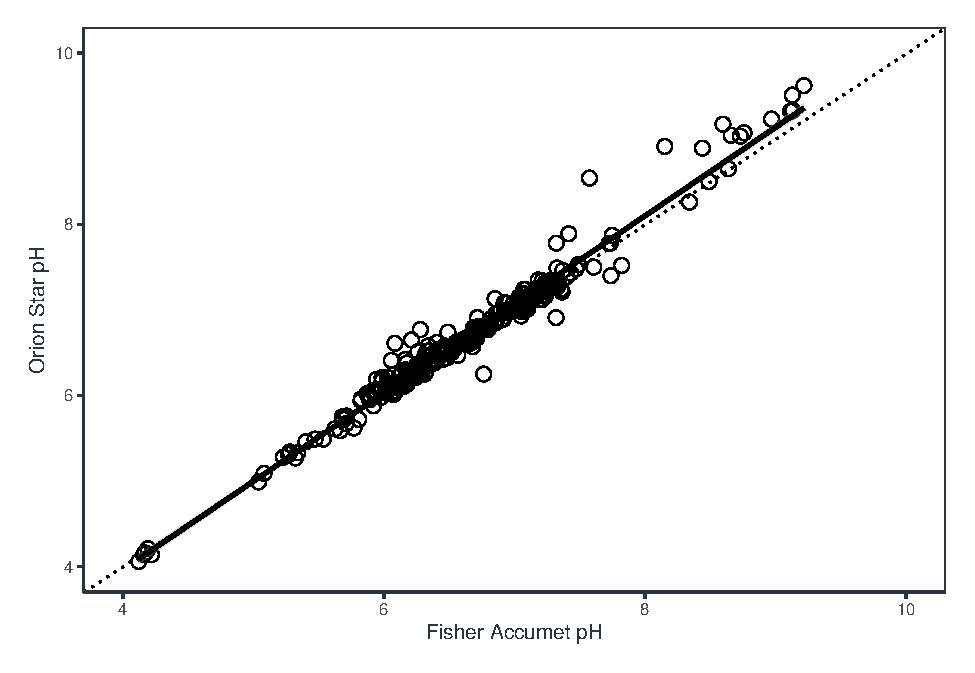
\includegraphics[width=0.5\textwidth]{fisher_v_orion.pdf}
  \caption{Comparison of pH results of samples measured on the Fisher Accumet pH meter and the Orion Star pH meter}
\end{figure}

\hypertarget{conclusions}{%
\subsection{Conclusions}\label{conclusions}}

\end{document}
